\documentclass[letterpaper, 10 pt, conference]{ieeeconf}  % Comment this line out if you need a4paper

%\documentclass[a4paper, 10pt, conference]{ieeeconf}      % Use this line for a4 paper

\IEEEoverridecommandlockouts
%%% PACKAGES
\usepackage{array} % for better arrays (eg matrices) in maths
%\usepackage{subfig} % make it possible to include more than one captioned figure/table in a single float
\usepackage{amsmath}
\usepackage{amssymb}
\usepackage{bbold}
\usepackage{mathtools}	
\usepackage{graphicx} % support the \includegraphics command and options
\usepackage{epstopdf}
\usepackage{caption}
\usepackage{subcaption}
\usepackage{color}
% \usepackage[usenames,dvipsnames]{xcolor}
\usepackage{multirow}
\usepackage{url}
\usepackage{booktabs}
% \usepackage{appendix}
\usepackage{placeins}
\usepackage{cases}
\usepackage{empheq}
\usepackage{picture}
\usepackage{calc}
\usepackage{xspace}

\newcommand{\pic}[2]{\includegraphics[width={#2}]{#1}}
%% Try this out


\newcommand{\na}{n/a{ }}
\newcommand{\eg}{e.g.}
\newcommand{\ie}{i.e.}

\newcommand{\Dm}{\ensuremath{\mathcal{D}_{-} }\xspace}





\title{Hardware Demonstration of Atomic Force Microscopy imaging via Compressive Sensing and $\mu$-path Scans}
\author{Academic Political Mine Field }

\date{\parbox{\linewidth}{\centering%
  %\today
\endgraf\bigskip
SOME project }}



%\date{} % Activate to display a given date or no date (if empty),
         % otherwise the current date is prined 

\begin{document}
\maketitle
\begin{abstract}A summary of the paper goes here.
\end{abstract}
\section{Introduction}

\section{Experimental Setup}
Our experimental setup consists of an Agilent 5400 AFM retrofitted with an nPoint 100A XY piezolectric stage. Through a breakout box, the Agilent 5400 provides access to the z-axis deflection signal and allows control of the z-axis piezo via a $\pm10$~v input on the standard control box. The Agilent hardware does not provide access to the z-axis stepper motor used for the course engagement, so we use the standard agilent software for this before setting it to open-loop mode.

All control logic is programmed into a Xilinx LX150 fpga inside a cRIO 9082 from National Instruments. The cRIO includes modular 16 bit analog-to-digital and digital-to-analog modules, capable of sample rates up to XXX-ksps and XXXmsps, respectively. In this paper, all control is done at 25~kHz, which is chosen based on the system dynamics.
\begin{figure}
% L B R T
  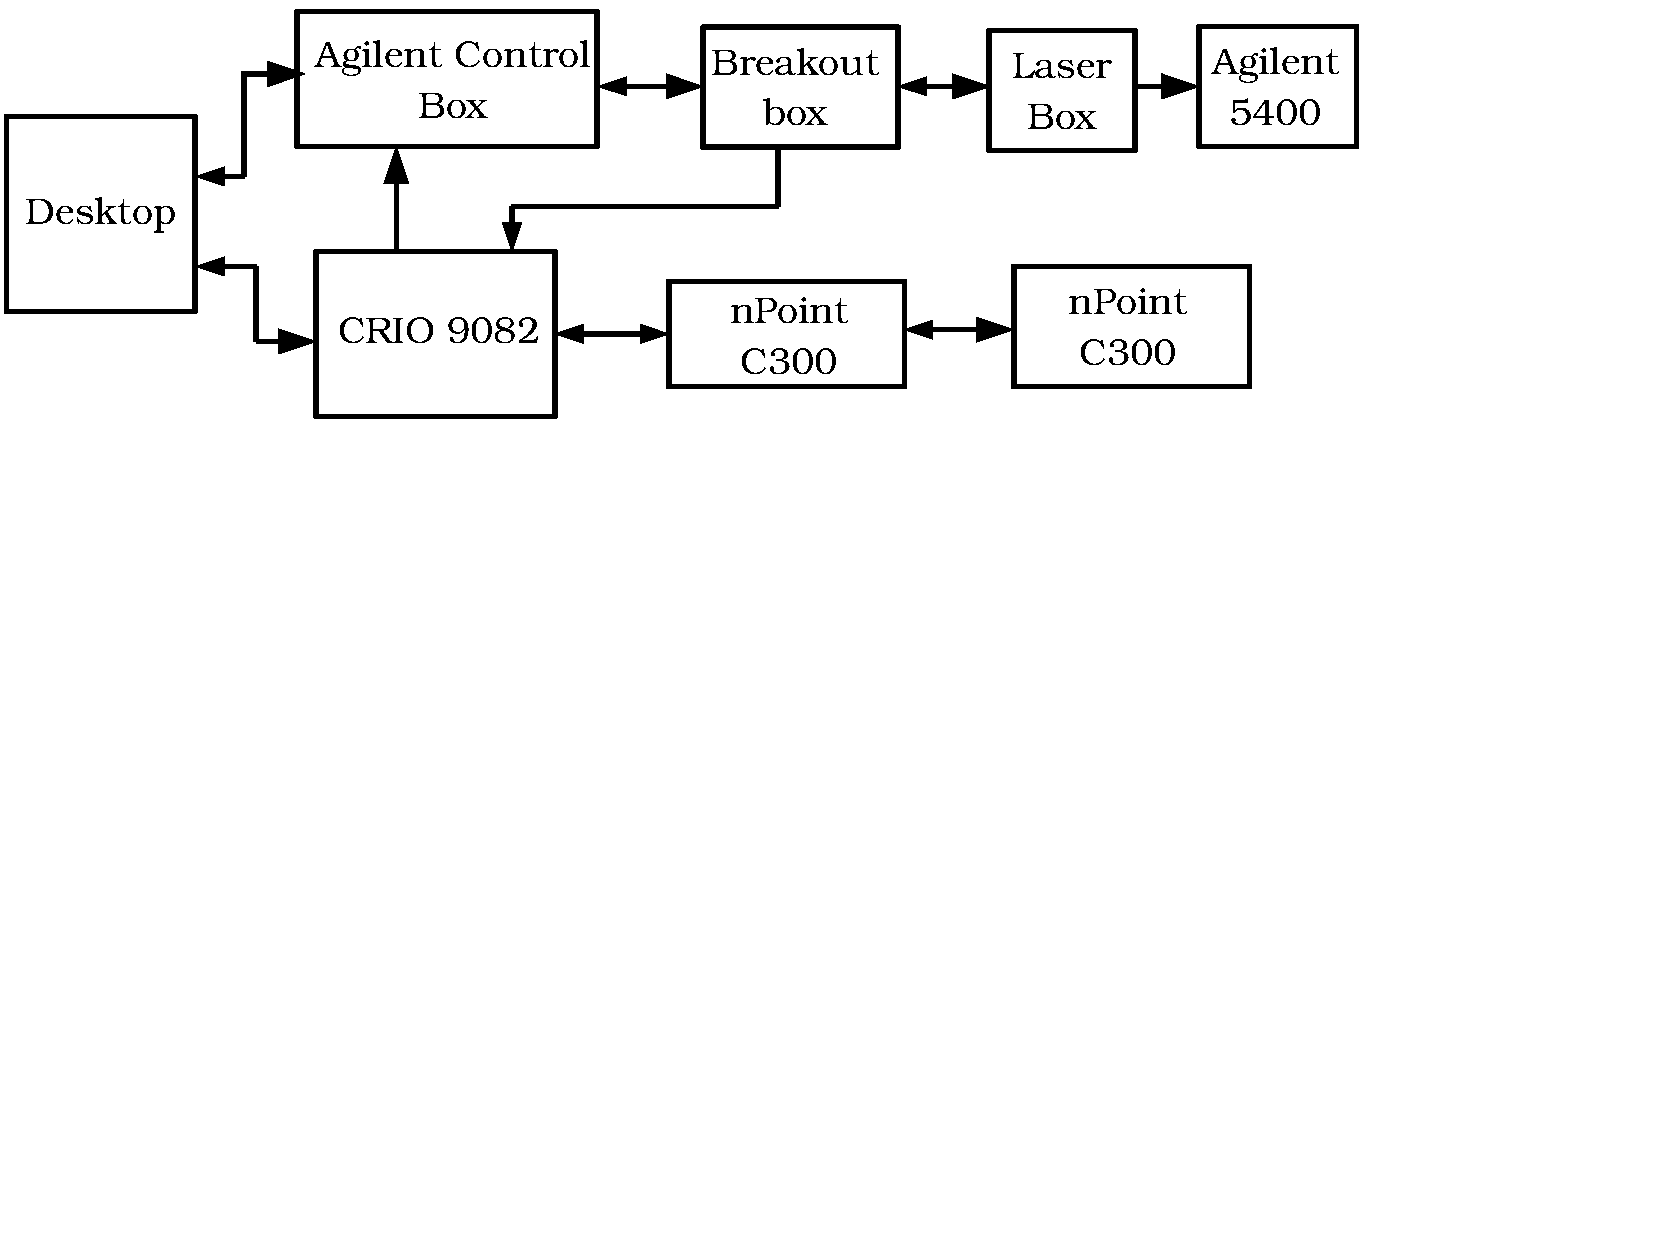
\includegraphics[trim=-00 350 0 0, clip,scale = .35]{figures/exp_setup}
  \caption{Schematic depiction of the experimental setup}
\end{figure}
\section{Implementation}
Implementing the $\mu$-path CS scheme involves several different distinct schemes. This is implemented as a simple state machine. For the $x$ and $y$ axis control loops, the state machine is only determining the reference signal. On the other hand, for the z-axis, the state machine is part of the control law itself, and part of its function to transition in and out of close-loop operation. 
\begin{enumerate}
\item{\textbf{initialization:}. You essentially always want to start in this state. The xy setpoint is nominally 0 (more on this in a bit). For our setup, you would turn off the agilent PI controller, and start up this vi. You then manually pull the tip away from the surface with the fron panel control `init Z up`.}
\item{\textbf{xy move:} In the first time step of this state, we read an $xy$ setpoint from the FIFO buffer and set $x_ref$ and $y_ref$ to those values. In subsequent time steps we do NOT read from the FIFO buffer, but just recycle that same setpoint. The trigger to move to the next state is a detection that the x(k) and y(k) have reached a settling criterion.}
\item{\textbf{Tip engagement}. This is comprised of two steps.
    \begin{enumerate}
    \item{\textbf{tip-lower} We now lower the tip towards the surface, at a rate determined by rate `ramp-rate`. Once the absolute value of the deflection (or error) signal exceeds `TOL`, that is the trigger to move to the next state.}
      \item{\textbf{z-axis PID}We now start PID control on the z-axis and wait for `|deflection(k) - setpoint|` to reach a settling criterion, which is the trigger to move to state 4.}

    \end{enumerate}
    }
\item{\textbf{measure} We initiate reading a trajectory path from the host-to-FPGA FIFO buffer, as well as start logging data into the fpga-to-host FIFO buffer. The xy-axis are now tracking some kind of trajectory, but our control here is agnostic to wheather this is a $\mu$-path, spiral scan, or discrete point. The trigger to move to the next state is that the xy trajectory we are following ends, which is determined by packing meta data into the host-to-FPGA FIFO data, which will be describe more fully in Section~\ref{sec:pack}}
\item{\textbf{tip-disengage} The xy PID control is set to the last value of the trajectory we were following, and we issue a step-up command to the z-axis control. For my hardware, I just wait `zup-N` samples, since I can't measure anything once the surface is disengaged. After `zup-N` samples we transition back to state 2.}
\end{enumerate}

\subsection{FIFO data packing}\label{sec:pack}
Data is transferred between the Host computer and the FPGA in real time via a Direct Memory Access (DMA) FIFO buffer. At each time step, the FPGA control law needs to acquire the current reference trajectory (state 4) or setpoint (state 2). Similarly, xy sensor measurements, z-error deflection data, and z-axis control data all need to be transferred back to the host. Because the FPGA is limited to a total of three DMA FIFO buffers, we pack the data together, transferring multiple pieces at each 40~$\mu$s time-step. Due to the possibility of a FIFO timeout, this is somewhat risky. On the one hand, if we wait on a piece of data too long, we violate the required sample time. On the other hand, setting a finite timeout brings the possibility of missing a piece of data. Timeout is partly mitigated by only transfering the interesting data---e.g., during the tip engagement, we do not transfer any data, which allows the host side time to catch and fill/empty the buffers. In the event that a timeout \emph{does} occur, the entire imaging process enters an abort routing. 

Furthermore, data traveling in both directions carries different meanings depending on which state it belongs to. To solve this dilemma, we transfer as well a piece of a meta data, which is just an integer coded to a meaning for that specific piece of data. 
\section{$\mu$-path description}

\section{Results}
In this study, we use a CS-20ng calibration grating. All features on the grating are 20~nm high. Although the grating has areas with several different sample patterns, here we use the area with a circles on a 500~nm pitch. The Agilent 5400 does not include a z-axis height sensor. In general, this makes it impossible to determine the relative heights between CS measurements. To work around this, we make the $mu$-paths 500 nm long, which ensures that if the scan starts on a feature, the scan must exit the feature, allowing us to register all CS measurements to a common height. 
\subsection{Timing Analysis}
\subsection{Density vs reconstruction}
\subsection{comparison to raster}
% \begin{center}
% \begin{tabular}{cccc}
% Region	   & $V_1^*$               & $V_2^*$           & $I_L^*$\\
% \hline
% \hline
% Dm 	   & $-\frac{R(G_b-G_a)}{1+RG_b}E$&	 $0$ 		& $\frac{(G_b-G_a)}{1+RG_b}E$\\
% Dz     & $0$		& $0$		& $0$\\
% Dp 	& $-\frac{R(G_a-G_b)}{1+RG_b}E$		& $0$		& $\frac{(G_a-G_b)}{1+RG_b}E$\\
% \hline
% \hline
% \end{tabular}
% \end{center}

% \begin{figure}
% \begin{subfigure}{.48\textwidth}
%   \includegraphics[angle=-90, origin=c,scale = 0.06]{figs_report/exp_period1}
%   \caption{Period one}
%   \label{fig:exp_period1}
% \end{subfigure}
% \begin{subfigure}{.48\textwidth}
%   \includegraphics[angle=-90, origin=c,scale = 0.06]{figs_report/exp_period2}
%   \caption{Period 2}
%   \label{fig:exp_period2}
% \end{subfigure}

% \end{figure}




% \bibliographystyle{IEEEtran}
% \bibliography{discreteLQR}
% \appendix
% \section{Appendix}\label{app:transform}



\end{document}


%%% Local Variables:
%%% mode: latex
%%% TeX-master: t
%%% End:
